\begin{problem}{체스판}{표준 입력(stdin)}{표준 출력(stdout)}{2\,초}{512\,MB}

건구스는 평소에 체스를 굉장히 좋아한다. 특히, 체스 말 중에서 나이트를 제일 좋아한다. 나이트는 아래 그림과 같이 특정 방향으로 2칸, 그와 직각인 다른 방향으로 1칸 떨어진 장소로 이동한다.

\begin{center}
  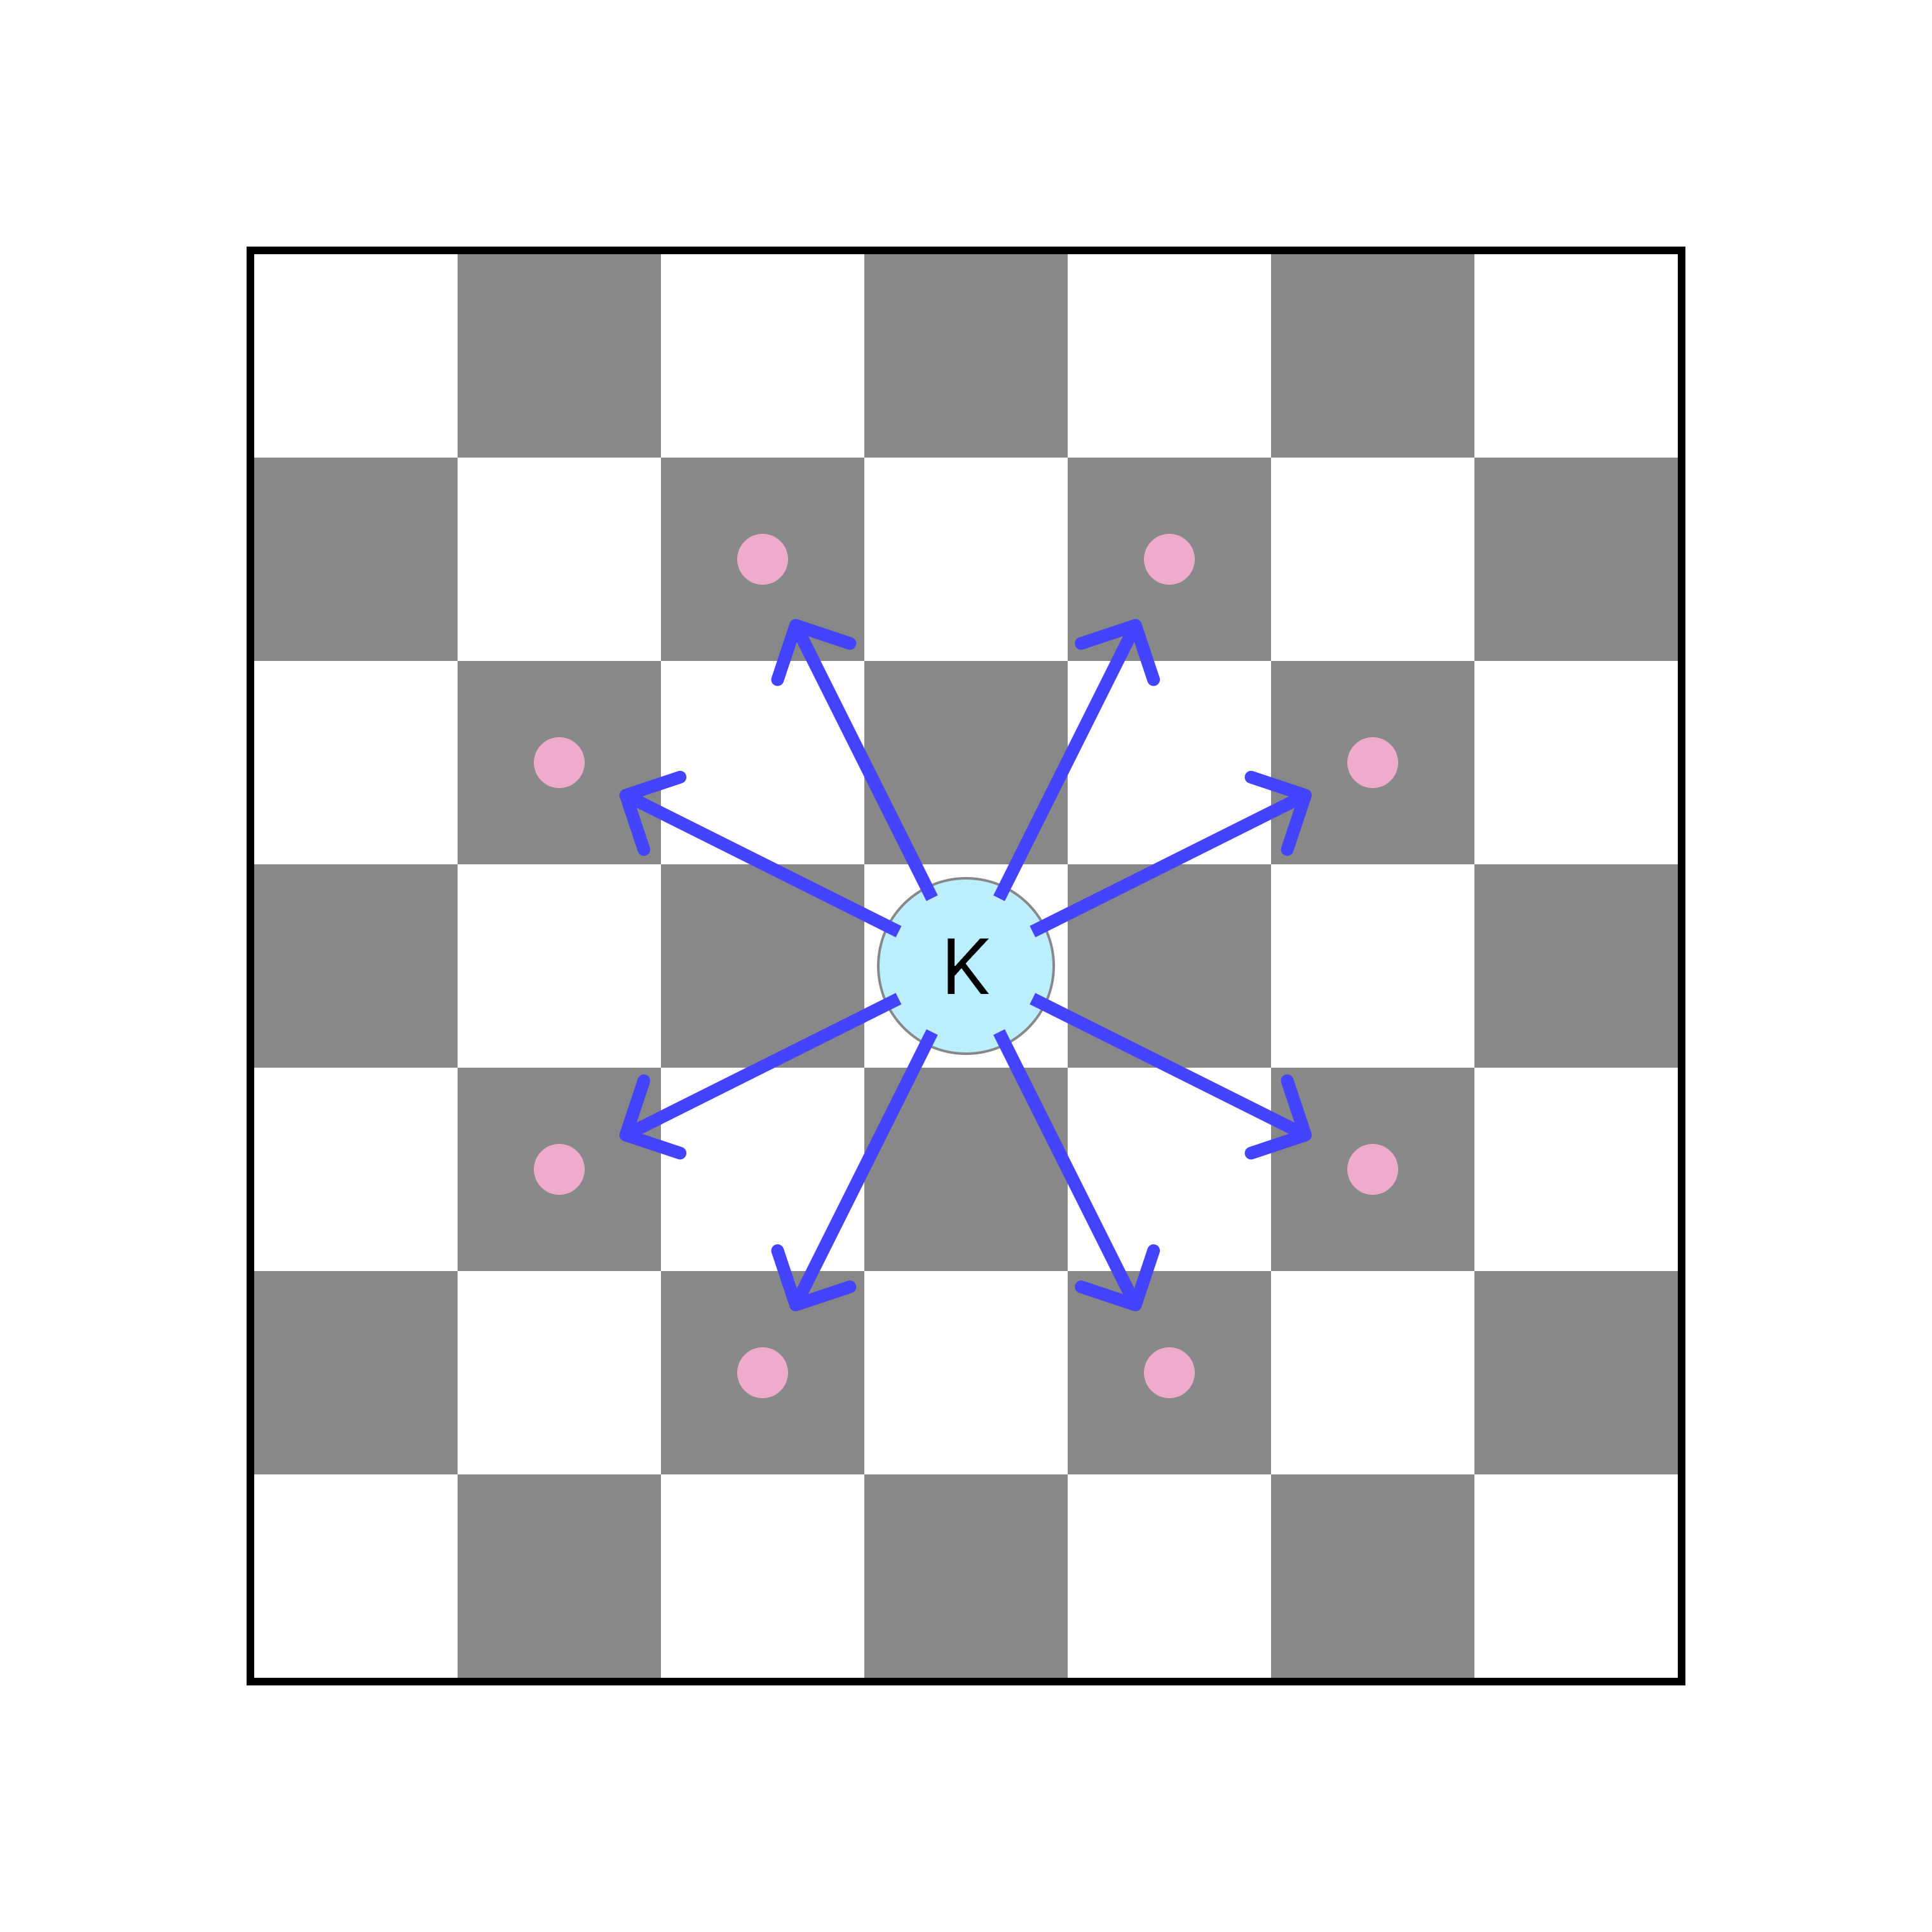
\includegraphics[width=0.4\textwidth]{../pictures/image1.png} \\
\end{center}

건구스는 어느 날 자면서 본인이 나이트가 되는 꿈을 꾸었다. 꿈속에서 자신이 무한히 넓은 체스판 위에 서 있다는 것을 알게 되었다. 건구스는 체스 말의 나이트처럼 움직일 수 있었고 재밌게 놀았다.
하지만, 꿈속에서 즐기다 보니 자신이 빨리 꿈에서 깨지 않으면 학교에 지각한다는 사실을 알게 되었다. 자신이 현재 $(x, y)$ 좌표에 있고, $(0, 0)$ 에 도착한다면 꿈에서 깰 수 있다.
건구스가 학교에 지각하지 않도록 가장 빨리 $(0, 0)$ 에 도착할 수 있는 방법을 알려주자!

체스판은 무한히 넓으며, $x$ 좌표나 $y$ 좌표가 음수인 칸에도 이동할 수 있음에 주의하자.
예시로 $(x, y)$ 가 $(2, 3)$ 인 경우, 최소 이동 횟수는 3이다.

\begin{center}
  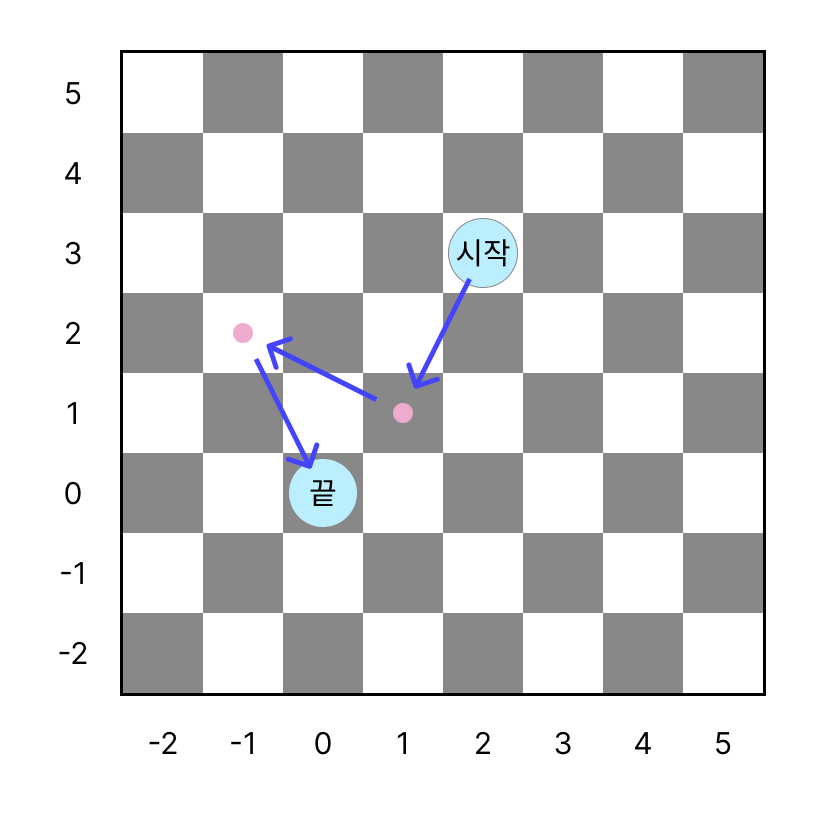
\includegraphics[width=0.4\textwidth]{../pictures/image2.png} \\
\end{center}

\InputFile
입력은 한 줄로 구성되어 있으며, 건구스의 좌표 $x$, $y$가 공백으로 구분되어 주어진다. $(0 \le x, y \le 1\,000)$

\OutputFile
첫째 줄에 $(x, y)$ 에서 $(0, 0)$ 으로 이동할 수 있는 최소 이동 횟수를 출력한다.

\Examples

\begin{example}
\exmp{
0 0
}{%
0
}%
\exmp{
1 0
}{%
3
}%
\exmp{
10 11
}{%
7
}%
\exmp{
1000 1000
}{%
668
}%
\end{example}

\end{problem}
